\subsection{Thematik}
Für den Prototypen bedarf es einer Thematik beziehungsweise einer Idee für das Gesamtkonzept. Dafür wurde die Idee einer \textit{Bienenkolonie} für interessant befunden. Bienen und deren Kolonien sind aus vielerlei Hinsicht geeignet als Thematik für den Prototyp, darunter der Fakt, dass Bienen bekannt dafür sind, Honig zu produzieren, wobei Honig eine konkrete Ressource darstellt. Im Kontext eines Resource Management Games und mit Rücksicht auf das zuvor untersuchte Spiel \textit{RimWorld} eignet sich jedoch am besten eine ganz spezifische Art der Bienen, die \textit{Honigbiene}, genauer gesagt die \textit{Westliche Honigbiene} (lat. \textit{apis mellifera}) \cite*[]{bees:name}. Grund dafür ist die Verhaltensweise von Honigbienen, da diese, anders als nahe Verwandte, stärker dazu tendieren, in Kolonien zu leben. Hummeln beispielsweise formen zwar auch Kolonien, aber deutlich kleinere und kürzer lebende. Die meisten Arten der Wildbienen jedoch sind tendenziell Einzelgänger. Eine weibliche Wildbiene legt ein Nest und versorgt ihren Nachwuchs mit Pollen und Nektar \cite*[]{bees:wild}. Somit bietet die Gattung der Honigbiene einige Vorgänge, welche sich in ein Colony Management Game umsetzen lassen. Dazu werden im Folgenden interessante Vorgänge und Eigenschaften der Gattung der Honigbiene genauer untersucht. Es ist zu erwähnen, dass der folgende Abschnitt nicht dazu dient, das gesamte Spektrum einer Bienenkolonie zu untersuchen, sondern lediglich Aspekte, die förderlich für die Entwicklung des Resource Management Games wären.

\subsubsection{Nahrung}
Eine Honigbiene ernährt sich primär von \textit{Nektar}, welchen sie von Blumen sammelt. Dieser Nektar ist zuckerhaltiger Saft, welcher von den Pflanzen ausgeschieden wird, um damit Insekten verschiedener Arten anzulocken. Dabei sind Sonnenblumen, Obstblüten, Löwenzahn und Raps besonders gute Nektarquellen \cite*[]{bees:food}. Eine weitere Möglichkeit um an energiereichen Zucker zu gelangen ist der sogenannte \textit{Honigtau}, welcher von einigen Insekten, darunter Blatt- und Schildläusen, ausgeschieden wird. Aus diesen beiden zuckerhaltigen Säften können die Bienen den \textit{Honig} produzieren, welcher ebenfalls als Nahrungsquelle dient, aber vor allem über die Wintermonate besonders wichtig ist, da Honig sehr lange haltbar ist \cite*[]{bees:honeywinter}. Der durch Honigtau produzierte Honig wird von Imkern als \textit{Waldhonig} gekennzeichnet \cite*[]{bees:food}. Saugt eine Biene den Nektar einer Blüte auf, gelangt dieser in den \textit{Honigmagen}. Dort kommt er in Kontakt mit verschiedenen Enzymen, welche den Nektar in \textit{Glukose} (Traubenzucker) und \textit{Fruktose} (Fruchtzucker) \cite*[]{bees:glucosefructose} aufspalten. Diesen biochemisch veränderten Nektar gibt die \textit{Sammelbiene} im Bienenstock an die sich dort befindlichen \textit{Arbeitsbienen} durch Auswürgen weiter, welche den Nektar erneut aufnehmen und auswürgen. Mit jedem dieser Prozesse wird der Nektar viskoser, wodurch allmählich Honig entsteht \cite*[]{bees:nectartohoney}.

Neben dem Nektar, dem Honigtau und dem Honig, welche primär als Quellen für Kohlenhydrate dienen, benötigen Bienen außerdem noch Quellen für Fette und Proteine. Dafür werden \textit{Pollen} verwendet, wobei Pollen die männlichen Geschlechtszellen einer Samenpflanze sind. Da die Samenpflanze mehr Pollen produziert, als für die Fortpflanzung nötig, können diese ohne Probleme von den Sammelbienen aufgenommen werden \cite*[]{bees:honeywinter}. Die Pollen werden in \textit{Pollenpaketen} aufbewahrt (vgl. \autoref{image:pollenpaket}), wobei Teile der aufgesammelten Pollen nicht in diesen Pollenpaketen landen, sondern an den Hinterbeinen haften bleiben. Besucht diese Sammelbiene nun eine weitere Blüte, werden diese Pollen abgestreift und der Fortpflanzungsmechanismus der Samenpflanze profitiert. Besonders pollenreiche Quellen sind dabei Obstbäume, Mohn, Mais, Klee und Raps \cite*[]{bees:honeywinter}.

\begin{figure}
    \begin{center}
        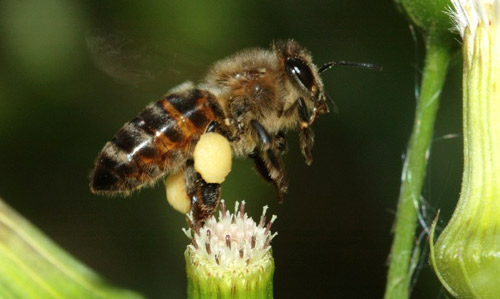
\includegraphics[width=300px]{0.bilder/pollenpaket.jpg}
    \end{center}
    \caption{Pollenpakete einer Honigbiene (\cite{bees:name})} \label{image:pollenpaket}
\end{figure}

Die letzte wichtige Ressource, welche Bienen für ihr Überleben benötigen, ist Wasser. Dieses kann von Flüssen oder Seen bezogen werden, wobei diese Quellen nicht mehr als 500 Meter weit vom Stock entfernt sein sollten. Erhalten Bienen nicht genug Wasser, können diese unter Verstopfungen leiden, was für das Überleben gefährlich sein kann \cite*[]{bees:honeywinter, bees:food}.

Es lassen sich somit wichtige Ressourcen identifizieren: \textit{Nektar, Honigtau, Honig, Pollen} und \textit{Wasser}. Außerdem ist die Aufteilung zwischen \textit{Sammel-} und \textit{Arbeitsbiene} eine mögliche Mechanik. Die Umwandlung von Nektar und Honigtau zu Honig könnte ebenfalls eine Mechanik darstellen, wie auch die naturgegebenen Quellen für Nektar, Honigtau und Pollen.

\subsubsection{Kasten}
Eine fundamentale Kategorisierung innerhalb einer Kolonie sind die \textit{Kasten}. Es gibt drei verschiedene Kasten beziehungsweise Arten von Bienen innerhalb solch einer Kolonie. Die erste Art ist die \textit{Bienenkönigin}. Diese Art der Biene ist genau ein mal vertreten und \textit{immer} ein Weibchen, zudem innerhalb einer Kolonie das einzige vollentwickelte. Die Hauptaufgabe der Königin ist das Brüten neuer Bienen und das Steuern des Schwarms mittels verschiedener Pheromone \cite*[]{bees:queen}. Die zweite Art sind die sogenannten \textit{Drohnen}. Diese Art ist \textit{ausschließlich männlich}. Diese Kaste ist lediglich zur Befruchtung der Königin da und ist nur von Frühling bis Sommer des Jahres in der Kolonie vertreten. Anschließend werden alle Drohnen gewaltsam aus der Kolonie entfernt, was als \textit{Drohnenschlacht} betitelt wird \cite*[]{bees:sex}. Die dritte und letzte Kaste der Kolonie sind die \textit{Arbeitsbienen}, welche, analog zur Königin, \textit{ausschließlich weiblich} sind, jedoch den deutlich größten Teil einer Kolonie ausmachen. Trotzdem legen diese Bienen in der Regel keine Eier, sind im Gegensatz dazu aber deutlich fürsorglicher gegenüber der Brut im Vergleich zur Königin. Die Arbeitsbienen sind prinzipiell für sämtliches weiteres Geschehen verantwortlich, darunter die Entfernung von Leichen oder die Nahrungsbeschaffung \cite*[S.2-3]{bees:frisch}. In \autoref{image:castes} werden die verschiedenen Kasten morphologisch unterscheidbar dargestellt mit einer Markierung verschiedener Merkmale. 

\begin{figure}
    \begin{center}
        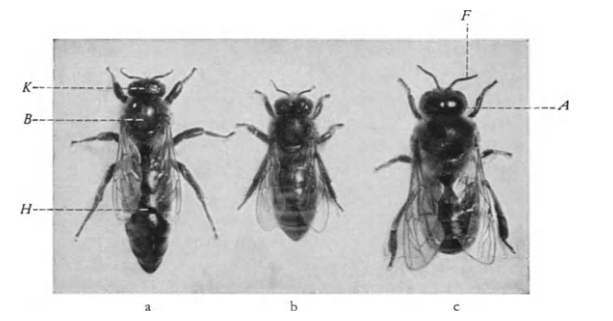
\includegraphics[width=300px]{0.bilder/castes.png}
    \end{center}
    \caption{(a) Königin, (b) Arbeitsbiene, (c) Drohne. (K) Kopf, (B) Brust, (H) Hinterleib, (A) Auge, (F) Fühler (\cite[S.2]{bees:frisch})} \label{image:castes}
\end{figure}



\subsubsection{Fortpflanzung}
Ein wichtiger Teil des Fortbestehens einer Kolonie ist die \textit{Vermehrung} beziehungsweise \textit{Fortpflanzung}. Wie bereits zuvor erwähnt gilt, dass sowohl Königinnen, als auch Arbeitsbienen jederzeit \textit{weiblich}, und Drohnen stets \textit{männlich} sind. Eine Königin ist in der Lage unbefruchtete Eier zu legen, oder diese Eier mittels Paarung mit Drohnen zu befruchten. Auch Arbeitsbienen sind in der Lage unbefruchtete Eier zu legen, was in einer Kolonie tendenziell selten passiert, da die Geschlechtsorgane der Arbeitsbienen zurückentwickelt und verkrümmt sind \cite*[]{bees:sex}. Wird allmählich eine neue Königin gebraucht, da die derzeitige Königin an das Ende ihres Lebens gelangt, sondert diese bestimmte Pheromone aus, wodurch dem Schwarm mitgeteilt wird, neue Königinnen heranzuziehen. Eine würde theoretisch ausreichen, aber um kein Risiko einzugehen werden mindestens \textit{sechs} Königinnen, oder mehr, versucht heranzuziehen. Nachdem eine geeignete Königin geschlüpft ist, werden die restlichen gewaltsam aus dem Schwarm entfernt \cite*[S.33]{bees:frisch}. Spätestens zwei Wochen später fliegt die neu geschlüpfte Königin aus und versprüht Pheromone, auch \textit{Königinnensubstanz} genannt, welche Drohnen eigener und fremder Völker anlocken, um sich mit der Königin zu paaren. Es wird mit maximal 12 Drohnen der Paarungsakt vollzogen, wobei die Königin bis zu \textit{zehn Millionen} Spermien aufnimmt, welche für die restliche Lebenszeit reichen \cite*[]{bees:queen}.

Einige Tage nachdem die Eier der zukünftigen Königinnen gelegt wurden, in der Regel neun Tage, beginnt der Akt des \textit{Schwärmens}. Dabei verlässt ein Teil der Kolonie, tausende von Bienen, zusammen mit der noch regierenden Königin den Schwarm, um sich auf die Suche nach einem neuen Zuhause zu machen und ein neues Bienenvolk zu gründen. Dieser Akt passiert in der Regel nur ein Mal pro Jahr, gegen Mai. \textit{Spurbienen} agieren als Späher und teilen Informationen über mögliche neue Heimatplätze. Laut Forschungen bedarf es 15 Spurbienen, welche dieselben Informationen über einen passenden Ort teilen, damit die Entscheidung gefällt wird \cite*[]{bees:swarm}. Dank der Pheromone der Königin bleibt der Schwarm während des Schwärmens stets zusammen \cite*[]{bees:queen}. 

Eine Königin besitzt einen \textit{diploiden} Chromosomensatz, dementsprechend \textit{2n = 32} Chromosomen. Die \textit{unbefruchteten} Eier werden von keinem zweiten Chromosomensatz ergänzt, wodurch die sich daraus entwickelnden Drohnen vorerst einen \textit{haploiden} Chromosomensatz besitzen, dementsprechend \textit{n = 16} Chromosomen in Summe. Diese werden jedoch nachträglich diploid, lediglich die Keimzellen bleiben haploid. Dadurch gilt, dass die anschließend diploiden Körperzellen der Drohne  \textit{homozygot} sind, da sie mittels \textit{Autopolyploidisierung} aus einer haploiden Eizelle entstanden sind. Beide Gene eines Merkmals stimmen also exakt überein \cite*[]{bees:homozygot}. Aus unbefruchteten Eiern schlüpfen ausschließlich Drohnen. Gegensätzlich dazu schlüpfen aus den \textit{befruchteten} Eiern Arbeitsbienen \textit{oder} Königinnen. Diese Eizellen sind durch die Beteiligung zweier Partien, der Königin und einer Drohne, sowohl \textit{heterozygot}, als auch diploid. Der Faktor, ob aus einem befruchteten Ei eine Arbeitsbiene oder eine Königin schlüpfen wird, ist modifikativ, also durch äußere Einflüsse, bestimmt. Der Unterschied liegt in der zugegebenen Nahrung der Maden in den ersten drei Lebenstagen. Während die zukünftigen Arbeitsbienen mit Pollen und Honig ernährt werden, erhalten die zukünftigen Königinnen ausschließlich \textit{Gelée Royal} (engl. \textit{Royal Jelly}) in ihren sogenannten \textit{Weiselzellen}, welche ausschließlich einer zukünftigen Königin vorenthalten sind \cite*[]{bees:swarm}. Somit gilt, dass Arbeitsbienen und Königinnen genetisch identisch sind, jedoch durch die zugegebene Nahrung modifikativ zu einer gewissen Kaste herangezogen werden können \cite*[]{bees:sex}. Es gilt also dass, auch wenn auf den ersten Blick paradox erscheinend, eine Drohne nie einen Vater, aber immer einen Großvater hat.

\subsubsection{Metamorphose}
Der Vorgang der \textit{Metamorphose} beschreibt das Anpassen der physischen Form oder ein plötzliches Ändern der äußeren Erscheinung \cite*[]{bees:metamorphosisdefinition}. Bienen durchlaufen vier verschiedene Zustände der Metamorphose, beginnend als \textit{Ei} (engl. \textit{egg}). Diese Eier werden von der Königin in eine leere Wabe gelegt, haben eine Größe von 1mm bis 1.5mm und ähneln einem Reiskorn. Nach circa \textit{drei Tagen} brechen die Eier und eine \textit{Larve} (engl. \textit{larva}) kommt hervor. Diese Larve ist weiß und C-förmig (vgl. \autoref{image:metamorphosis}). Die Dauer der kommenden Metamorphose hängt von der jeweiligen Kaste der zukünftigen Biene ab, Arbeitsbienen benötigen 6 Tage, Drohnen 6.5 Tage und Königinnen 5.5 Tage. Ist die Larve reif für die Metamorphose, richtet sie sich auf, sodass die Arbeitsbienen, welche Zuständig für die Brut sind, die Zelle mit \textit{Bienenwachs} bedecken. Die Larve verhärtet und wird zu einer \textit{Puppe} (engl. pupa). Analog zum vorherigen Stadium ist die Dauer bis zur kommenden Metamorphose abhängig von der Kaste der zukünftigen Biene. Eine Arbeitsbiene benötigt 12 Tage, eine Drohne 14.5 Tage und eine Königin 8 Tage. Ist die Zeit reif und die Metamorphose abgeschlossen beißt sich die Biene durch das Bienenwachs der Zelle und gesellt sich zu ihren Artgenossen \cite*[]{bees:name}.


\begin{figure}
    \begin{center}
        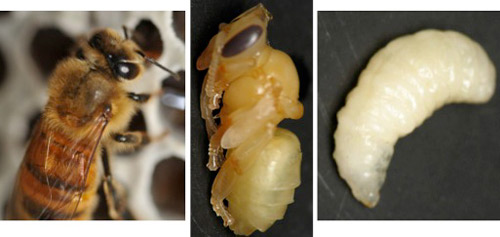
\includegraphics[width=300px]{0.bilder/metamorphosis.jpg}
    \end{center}
    \caption{Verschiedene Stadien einer Honigbiene, ausgewachsen (links), Puppe (mitte), Larve (rechts) (\cite[]{bees:name})} \label{image:metamorphosis}
\end{figure}

\subsubsection{Aufgabenverteilung}
Die Aufgaben der Königin und der Drohnen wurde zuvor bereits ausgiebig erläutert.
Eine Arbeitsbiene hat drei exakt eingeteilte Phasen ihres Lebens, in welchen verschiedene Tätigkeiten verrichtet werden. Die zu erledigenden Aufgaben sind also direkt gekoppelt an das derzeitige Alter einer Arbeitsbiene. Der erste Lebensabschnitt ist zwischen dem 1. und 10. Lebenstag der Biene. In diesem Stadium wird die Biene als \textit{Hausbiene} bezeichnet, da sie sich 
ausschließlich innerhalb des Bienenstocks aufhalten. Dort reinigen sie die Zellen, kümmern sich um die Brut als sogenannte \textit{Brutamme} und sind ansonsten meist untätig. Der zweite Lebensabschnitt findet zwischen dem 10. und 20. Lebenstag der Biene statt. In diesem Abschnitt wird die Biene als \textit{Baubiene} eingestuft. Die Aufgaben sind nun primär das Entgegennehmen des von den Sammlern gebrachten Nektar oder der Pollen, das Bauen neuer Waben und das Herstellen von Wachs. Außerdem sind manche diese Bienen im \textit{Wächterdienst} und beschützen den Stock vor Eindringlingen wie Wespen, Pferden oder Menschen. Im dritten und letzten Abschnitt des Lebens sind die Bienen \textit{Sammlerbienen}, welche Nahrung für den restlichen Stock von der Außenwelt suchen. Allerdings gibt es nur Ausflüge, wenn das Wetter und die Temperatur passend sind. Bei Regen, Schnee oder generell im Winter sitzen diese Bienen im Stock und warten auf Veränderung der Außenbedingungen. In der Regel widmen diese Bienen sich nicht den anderen Aufgaben und warten stattdessen \cite*[S.42-44]{bees:frisch}. \autoref{image:livesofcastes} zeigt einen Überblick der jeweiligen Aufgaben abhängig von dem Alter einer Biene jeglicher Kaste.

\begin{figure}
    \begin{center}
        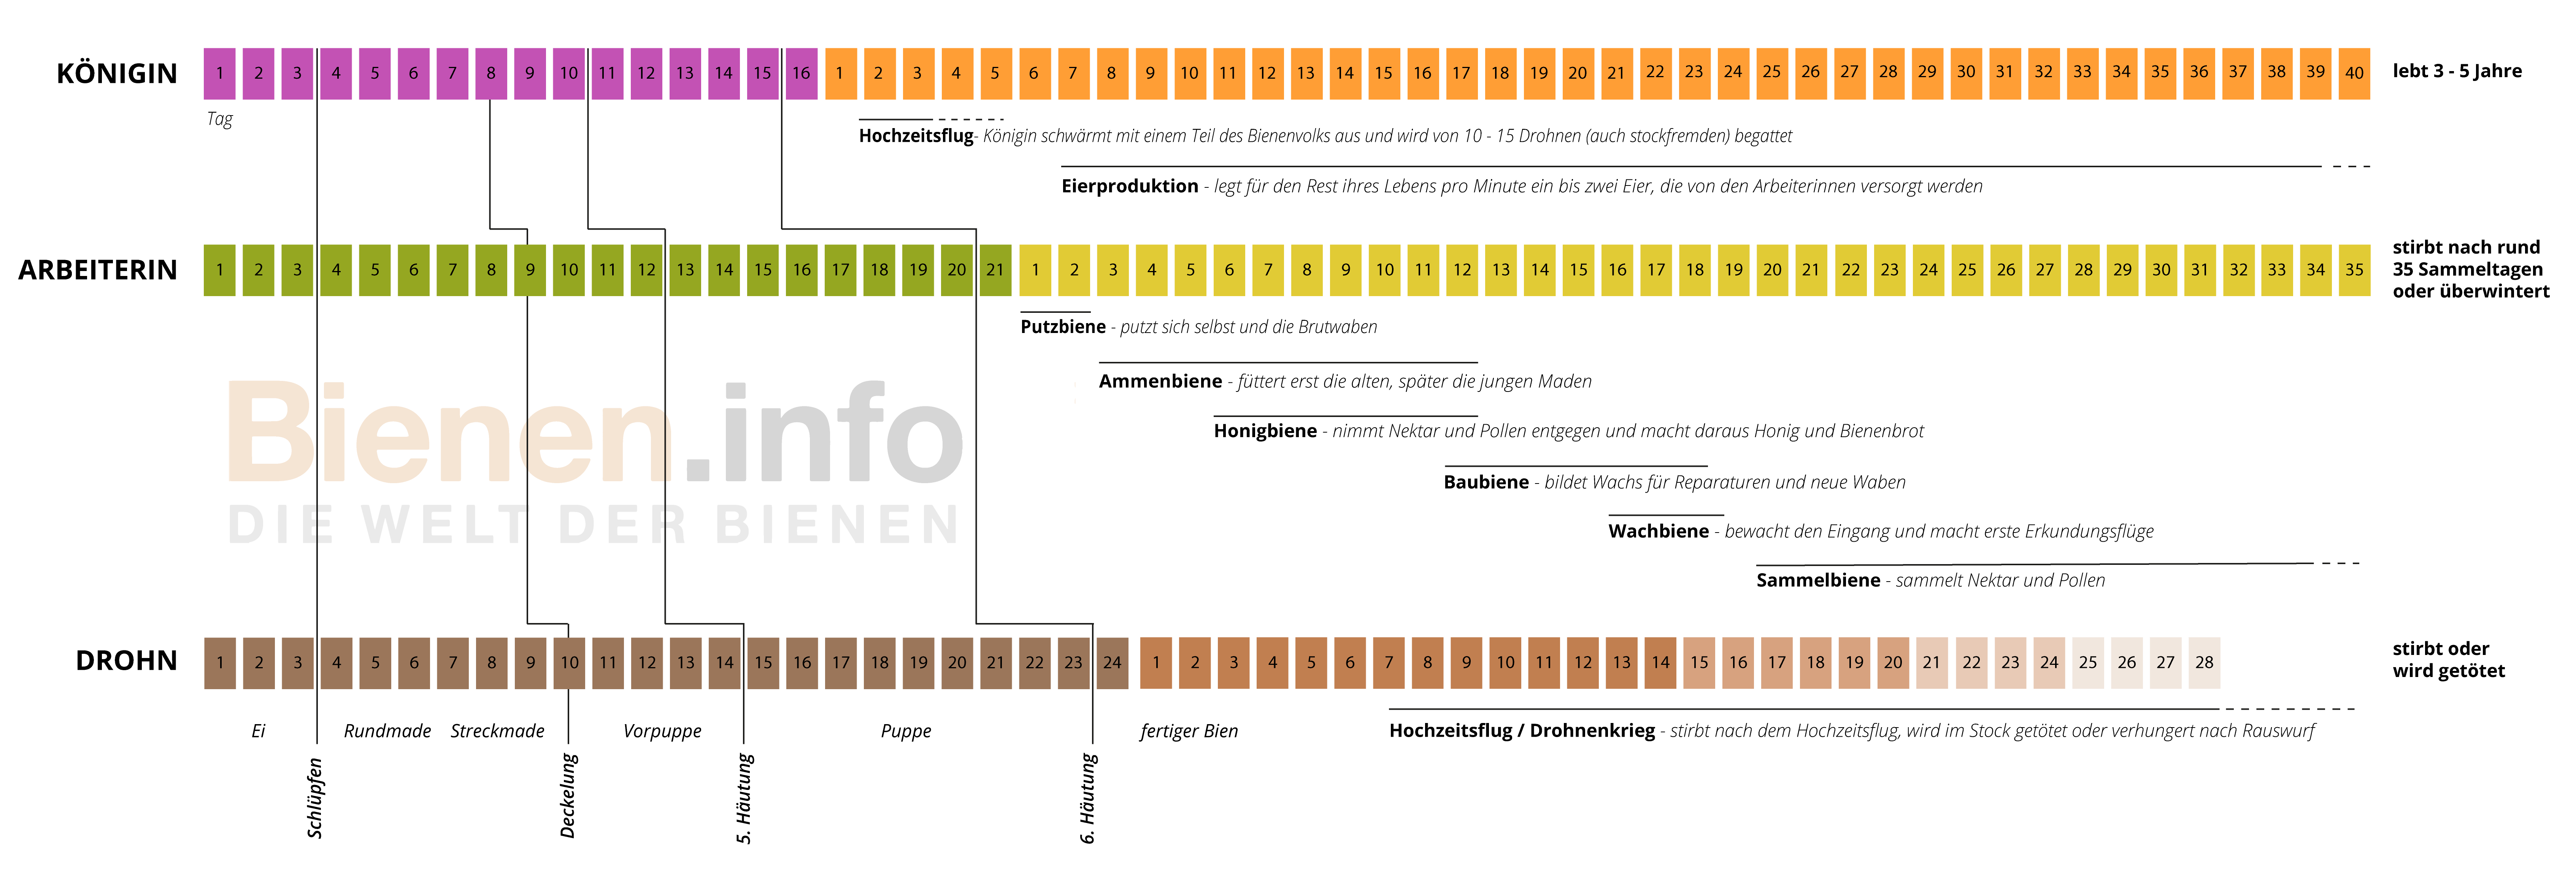
\includegraphics[width=400px]{0.bilder/livesofcastes.png}
    \end{center}
    \caption{Überblick über den Lebensverlauf einer Biene jeder Kaste (\cite[]{bees:lifeexpectancy})} \label{image:livesofcastes}
\end{figure}


\subsubsection{Lebenserwartungen}
Die Lebenserwartung einer jeden Biene hängt mit ihrer jeweiligen Kaste zusammen. Die kürzeste Lebensdauer weisen die Drohnen auf, welche zwischen zwei bis vier Wochen leben, da diese anschließend durch die Drohnenschlacht gewaltsam entfernt oder getötet werden. Am längsten hingegen leben Königinnen, mit drei bis fünf Jahren Lebensdauer. Bei Arbeitsbienen ist es entscheidend, ob diese während des Sommers oder gegen Anbruch des Winters geschlüpft sind. Durch die Wintereinnistung steigt die Lebenserwartung der Arbeitsbienen stark an, von gerade mal zwei bis vier Wochen auf sechs bis sieben Monate \cite*[]{bees:lifeexpectancy}. Eine Übersicht dieser Lebenserwartungen ist in \autoref{image:lifeexpectancy} vorzufinden.

\begin{figure}
    \begin{center}
        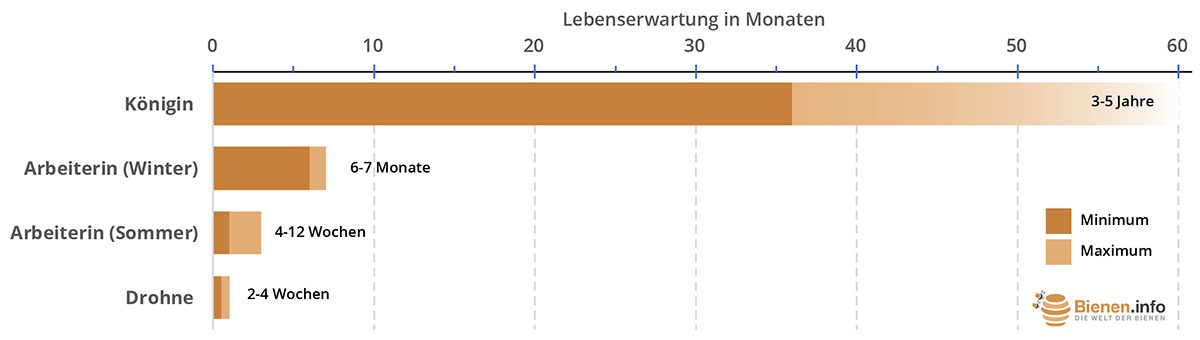
\includegraphics[width=400px]{0.bilder/lifeexpectancy.png}
    \end{center}
    \caption{Die minimale und maximale Lebenserwartung einer Biene jeder Kaste (\cite[]{bees:lifeexpectancy})} \label{image:lifeexpectancy}
\end{figure}

\subsubsection{Winter}
Die Vorbereitung auf den kommenden Winter beginnt bereits im Spätsommer, wobei neue Brut erzeugt wird für den Zweck der Überwinterung, sogenannte \textit{Winterbienen}. Ab Oktober werden die \textit{Sommerbienen} aus der Kolonie entfernt, sodass die Kolonie lediglich aus Winterbienen besteht. Dadurch, dass keine Energie für Brutpflege oder Sammelflüge aufgewendet werden muss, ist die Lebenserwartung der Winterbienen deutlich höher als die der Sommerbienen, wie bereits zuvor erläutert. Außerdem legen sich die Winterbienen ein Fettpolster zu, durch hohen Konsum von Pollen. Statt eines Winterschlafes formiert sich der Stock zu einer \textit{Wintertraube}, bei welcher die Kolonie die Königin umschließt und durch Muskelvibration warm hält. Mit Anfang des Frühlings wird mit gleicher Technik der Stock auf 35°C erhitzt, wodurch der Nahrungsverbrauch stark ansteigt aber das erfolgreiche Brüten der neuen Generation sichert. Sobald die ersten Blumen wieder sprießen setzen wieder die Sammelflüge ein \cite*[]{bees:winter}.